\documentclass[10pt]{seminar} 

\renewcommand{\baselinestretch}{1}

\usepackage{amsmath}

\renewcommand{\printlandscape}{\special{landscape}}

\usepackage{ulem}



\input{seminar.bug}

%\usepackage{fancybox}

\usepackage{epsfig}

%\usepackage{times}


\usepackage{amssymb}

\usepackage{amscd}

\usepackage{graphics}

\usepackage{pstricks}

%\usepackage{chicago}

%\usepackage{fullpage}

\slideframe{none}

\begin{document}

\newtheorem{proposition}{Proposition}

\newtheorem{definition}{Definition}

\newtheorem{corollary}{Corollary}

\newtheorem{theorem}{Theorem}

\newtheorem{lemma}{Lemma}

\def\argmax{\mathop{\rm argmax}\limits}  


%\slideframe{Oval}

\sffamily 


\begin{slide}
\begin{center}
Sets \& Functions \small
 

 \end{center}
 
 \newslide
 A ``collection of objects viewed as a single entity" is called a \textit{set}
 
 \vspace{.25in}
 \begin{itemize}
 \item If the objects in the set can be counted then it's common for the set to be written by enclosing the objects in curly braces $\{...\}$
 
 \begin{itemize}
 \item The curly braces are extremely important: $\{1, 4, 5\}\not=(1, 4, 5)$
 \end{itemize}
 
 \item Examples of sets: $\{$Maggie, Bobby$\}$, or $\{2, 5, 3, 8, 10\}$, or \\$\{$red, green, blue$\}$
 
 \item The elements of a set must all be unique: $\{1, 1, 3, 4, 4\}$ is not a set \\(it's a \textit{multiset})
 \item The ordering of elements in a set does not matter: \\$\{$red, blue, green$\}$=$\{$green, blue, red$\}$
 \end{itemize}
 \newslide
 
 Basic and essential notation involving sets
 
  \begin{itemize}
 \item ``Is an element of " is $\in$
 \begin{itemize}
 \item green $\in \{$red, green, blue$\}$
  \item magenta $\not\in \{$red, green, blue$\}$
   \end{itemize}
  
 \item ``Is a subset of" is $\subset$
 
  \begin{itemize}
 \item $\{$green, red$\} \subset \{$red, green, blue$\}$
  \item Note that green $\not\subset \{$red, green, blue$\}$ because ``green" is not a set!
    \item However $\{$green$\}\subset \{$red, green, blue$\}$ because $\{$green$\}$ IS a set
    \item Sometimes a distinction is made between $\subset$ (strict subset) and \\ $\subseteq$ (weak subset); your book doesn't make the distinction
   \end{itemize}
 
\newslide

\item ``Union" is $\cup$, and represents the set of elements in \textit{either} set
\vspace{.25in}
\begin{itemize}

\item $\{$Maggie, Bobby$\} \cup \{2, 5, 3, 8, 10\}$ \\ =$\{$Maggie, Bobby$, 2, 5, 3, 8, 10\}$
\vspace{.15in}
\item $\{$Maggie, Bobby$\} \cup \{2, 5, 3, 8, 10\} \cup \{$red, green, blue$\}$ \\ $=\{$Maggie, Bobby$, 2, 5, 3, 8, 10$, red, green, blue$\}$
\vspace{.15in}
\item $\{$Maggie, Bobby$\} \cup \{$Maggie, Bobby$\} =\{$Maggie, Bobby$\}$
\end{itemize}

\newslide

\item ``Intersection" is $\cap$, and represents the set of elements in \textit{both} sets
\vspace{.25in}
\begin{itemize}

\item $\{$Maggie, Bobby$\} \cap \{$Bobby, Bogdan$\}$=$\{$Bobby$\}$

\item $\{$Maggie, Bobby$\} \cap \{2, 5, 3, 8, 10\}=\emptyset$

\end{itemize}

\vspace{.05in}

\item $\emptyset$ is the ``empty set" which is the set that contains nothing, or $\{\}$ 
\vspace{.05in}
\item The output of union and intersection operations \textit{is always a set}!

\begin{itemize}
\item $\{$Maggie, Bobby$\} \cap \{$Bobby, Bogdan$\} \not=$ Bobby
\end{itemize}

\item If two sets have an empty intersection, they are \textit{disjoint}

\begin{itemize}
 \item $\{$Maggie, Bobby$\}$ and $  \{2, 5, 3, 8, 10\}$ are disjoint
\end{itemize}

 \end{itemize}
 
  \newslide
Oftentimes we don't want to (or can't) simply list all the items in a set, so we define sets in other ways (note  we \textit{always use the curly braces})

\vspace{.15in}
\begin{itemize}
\item The set of all the boys' names that start with a vowel: $\{x: x\hbox{ is a boy's name starting with a vowel}\}$

\item The set of all real numbers greater than -17.5 and less than 4: $\{x\in \mathbb{R}:-17.5<x<4\}$
\end{itemize}
 
 Using this kind of notation, we can define the following:
 
 $$A\cup B=\{x: x\in A \hbox{ or } x\in B\}$$
 
 $$A\cap B=\{x: x\in A \hbox{ and } x\in B\}$$
 

 
\newslide

Claim:  The empty set $\emptyset$ is a subset of every set.

\ \\\underline{Direct proof}: First, note that $B\subset A$ is equivalent to the statement that $$\forall x\in B \hbox{ we have }  x\in A.$$ 

We want to prove that $\emptyset \subset A$ for any set $A$.

This is equivalent to saying that for all $x\in \emptyset$, we have $ x\in A$.  But we know that $\not\exists x\in \emptyset$.  Therefore the statement that these (nonexistent) $x$ are in $A$ is vacuously true.  $\Box$

\newslide
Conditional statements \& vacuous truths

\ \\Claims of the form $A\Rightarrow B$ are \textit{conditional statements}

\begin{itemize}
\item ``If $A$ is true then $B$" is true
\item $A$ is the \textit{antecedent} and $B$ is the \textit{consequent}
\item $A\Rightarrow B$ is false \textit{only when} $A$ is true and $B$ is false 
\item If antecedent $A$ isn't true then the conditional statement is \textit{vacuously true}
\end{itemize}


\newslide
Other vacuously true statements:

\ \\ \underline{Claim}: If the moon was purple, then rain would fall up.

\vspace{.2in}

\underline{Definition}: A binary relation is \textit{quasitransitive} if $a>b$ and $b>c$ implies that $a>c$.

\underline{Claim}: The binary relation with $a=b$ and $b>c$ and $a=c$ is quasitransitive.

\newslide

Claim:  The empty set $\emptyset$ is a subset of every set.

\ \\\underline{Proof by contradiction}: First, note that $B\not\subset A$ is equivalent to the statement that $$\exists x\in B \hbox{ such that } x\not\in A. $$

Suppose that $\emptyset \not\subset A$.  Then by the above statement we know that $\exists x\in \emptyset: x\not\in A$.  However, this contradicts the fact that $\not\exists x\in \emptyset$.  Thus, $\emptyset\subset A$.   $\Box$

\newslide More definitions

\begin{itemize}
\item A \textit{family of sets} is a set whose elements are themselves sets

\begin{itemize}
\item $\{\{1, 2, 4\}, \{2, 6\}, \{\hbox{green}\}\}$
\end{itemize}
\item A well-known family of sets is the \textit{power set} of any set $X$: it is the set of all subsets of $X$, and is written $2^X$ 
\begin{itemize}
\item $2^{\{\hbox{cat, dog}\}}=\{\emptyset, \{\hbox{cat}\}, \{\hbox{dog}\}, \{\hbox{cat, dog}\}\}$
\end{itemize}
\item $|X|$ is the cardinality (size) of set $X$; the number of elements in $X$
\begin{itemize}
\item If $|X|=n$ then $|2^X|=2^n$

\end{itemize}

\newslide
Quick aside on proof strategies:

\ \\Proof by contradiction: We want to show $A\Rightarrow B$.  Assume that both $A$ and $\neg B$ hold simultaneously.  Show that this implies a contradiction.

\ \\Proof by contrapositive: We want to show $A\Rightarrow B$.  Prove that $\neg B \Rightarrow \neg A$.

\ \\Proof by induction: We want to show that a property holds for all $n$, where $n$ is an integer.  (1) Prove it holds for $n=0$ (or $n=1$).  (2) \textit{Assume} it holds for arbitrary $n$.  (3) Prove it must hold for $n+1$.

\newslide



Claim:  If $|X|=n$ then $|2^X|=2^n$

\ \\\underline{Proof by induction}: Suppose that $|X|=0$.  If $X$ has no elements, then $X=\emptyset$. It follows that  $2^{\{\}}=\{\{\}\}$: the set of all subsets of $\emptyset$ is just the set containing $\emptyset$.  Thus, $|2^{\{\}}|=2^{|X|}=2^0=1$, proving our statement for $n=0$.

\ \\Suppose our statement holds for $|X|=n$, so $|2^X|=2^n$.  

\ \\Let $Y=X\cup \{x\}$, so that $|Y|=n+1$.  $2^Y$ is $2^X\cup\{S: S\subset Y \text{ and } x\in S\}$.  Note that $2^X$ and $\{S: S\subset Y \text{ and } x\in S\}$ are disjoint.

\ \\The set $\{S: S\subset Y \text{ and } x\in S\}$ has $2^n$ elements: it is $\{S:  S=\{x\}\cup Z \text{ where } Z\in 2^X\}$.  Thus, $|2^Y| = 2^n+2^n=2*2^n=2^{n+1}$. This proves our result. $\Box$

\newslide

\item If $A\subset B$ then the set of things that are in $B$ but not $A$ is the \textit{complement of $A$ in $B$}

$$B\setminus A= \hbox{ The complement of $A$ in $B$} = \{x\in B: x\not\in A\}$$

\item A set with a finite number of elements is a finite set

\item A set with an infinite number of elements is an infinite set
\end{itemize}



\newslide Sets of numbers

\begin{itemize}
\item The real numbers, $\mathbb{R}$: All numbers that are positive, negative, or 0

\item The natural numbers, $\mathbb{N}$: The set of all strictly positive integers \\$\mathbb{N}=\{1, 2, 3, 4, ...\}$

\item The integers, $\mathbb{Z}: $ the natural numbers, their negatives, and 0\\$\mathbb{Z}=\{..., -2, -1, 0, 1, 2 ...\}$

\end{itemize}

\newslide

Ordered lists

\begin{itemize}
\item  Unlike sets, \textit{ordered lists} are denoted with smooth brackets $(c, a, b, d, e)$
\begin{itemize}
\item Elements can repeat
\end{itemize}
\item The 2-dimensional plane is represented by $\mathbb{R}^2$, or $\mathbb{R}\times \mathbb{R}$


$$\mathbb{R}^2=\{(x, y): x\in \mathbb{R} \hbox{ and }y\in \mathbb{R} \}$$

\end{itemize}


\newslide
Cartesian product

\begin{itemize}
\item The general idea of an ordered pair doesn't require it to consist of two real numbers (or even two elements  of the same set!)

\item Given two sets $X$ and $Y$, the Cartesian product of $X$ and $Y$ is $\{(x, y): x\in X \hbox{ and }y\in Y\}$

\begin{itemize}
\item $\{\hbox{cat, dog}\}\times \{a, b\}= \{(\hbox{cat}, a), (\hbox{cat}, b), (\hbox{dog}, a), (\hbox{dog}, b)\}$
\end{itemize}

\item $X_1\times X_2\times ... \times X_n=\{(x_1, x_2, ..., x_n):x_i\in X_i \hbox{ for }i=1, 2, ..., n\}$

\item $\mathbb{R}^n$ is the $n$-ary Cartesian product of $\mathbb{R}$
$$\mathbb{R}^n=\{(x_1, x_2, ..., x_n): x_i\in \mathbb{R} \}$$


\newslide

\item An ordered list of numbers is a \textit{vector}
\item If the vector has $n$ elements, then it is an element of $n$-dimensional Euclidean space, or $\mathbb{R}^n$

\begin{itemize}
\item $(1, 5, 7)\in \mathbb{R}^3$
\item $(3, 2, 7, 12, 65, 78787, 3)\in \mathbb{R}^7$

\end{itemize}
\item If $n\leq 3$, you can plot out the vector (as either on a line, the plane, or 3-D space)
\item If $n>3$ you can't plot the vector out, but there is no other conceptual difference


\end{itemize}


\newslide 

Functions

\begin{itemize}
\item A \textit{function} is a mapping from a set $X$ into a set $Y$ 
\item This means that for each element of $X$, $f$ assigns an element of $Y$, or $f: X\rightarrow Y$
\item The \textit{graph} of a function from $\mathbb{R} $ to $\mathbb{R}$ is the set $$\{(x, y)\in \mathbb{R}^2: y=f(x)\}$$

\end{itemize}

\newslide

A function $f: X\rightarrow Y$ is \textit{one-to-one} (or injective) if every element of $X$ maps into a unique element of $Y$ ($f(a)=f(b)\Rightarrow a=b$)


\ \\A function $f: X\rightarrow Y$ is \textit{onto} (or surjective) if every element of $Y$ is mapped into by some element of $X$ ($\forall y\in Y, \exists x\in X: f(x)=y$)

\ \\ A function that is one-to-one and onto is bijective

\begin{center}
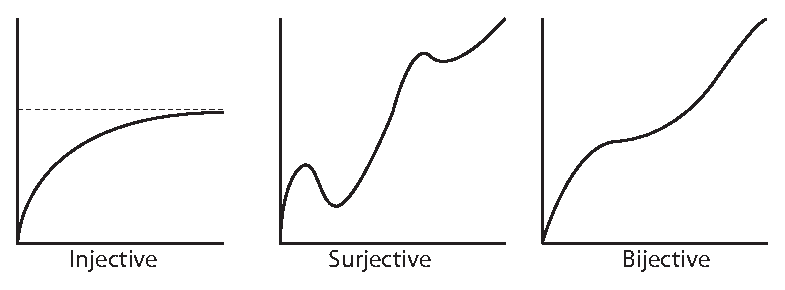
\epsfig{file=injective.eps, scale=.65}
\end{center}


\newslide

Composite functions

\begin{itemize}
\item Mappings can be combined so that if $f:B\rightarrow C$ and $g: A\rightarrow B$ then $f\circ g = f(g(x))$ is a mapping from $A$ to $C$

\begin{itemize}
\item $x\in A$, $g(x)\in B$, and $f(g(x))\in C$
\end{itemize}
\end{itemize}

Example: 

$f: \mathbb{R}^2\rightarrow \mathbb{R}$, with $f(x, y)=x+2y$

$g: \mathbb{R}^3\rightarrow \mathbb{R}^2$, with $g(x, y, z)=(x^2+2y*z, 7)$

$$h=f(g): \mathbb{R}^3\rightarrow\mathbb{R}, \text{ with }$$
$$h(x, y, z)=x^2+2y*z+14$$


\newslide

In-class problems

\begin{itemize}


\item[3.1.2] Let $A, B, C$ be sets such that $A\subset B$ and $A\cap C=\emptyset$.  Simplify the following, if possible:

\begin{itemize}
\item $A\cap(B\cup C)$ %A
\item $(A\cap B)\cup C$ % A\cup C
\item $A\cup(B\cap C)$ %No simplification 
\item $(A\cup B)\cap C$ %B\cap C


\end{itemize}

\newslide

\item[3.4.1] Let $f:\mathbb{R}^2\rightarrow \mathbb{R}^2$. Interpret the mapping $f(x, y)=(x, -y)$ geometrically
\begin{itemize}

\item Which points remain unchanged under this mapping? %It's the reflection about the x-axis.  The x-axis is unchanged.

\item Now answer both questions for $f(x, y)=(x, -4)$ % Projection onto line y=-1. Unchanged points are along the line y=-4.

\end{itemize}


\end{itemize}

\end{slide}




\end{document}








